\section{Defenses}
\subsection{KNN Sanitization Baseline}
We evaluated K-Nearest Neighbors (KNN) Sanitization, which replaces each context row with the geometric mean of its $K$ nearest neighbors. While intuitive, this defense was surprisingly ineffective. At $K=3$, the MSE only dropped from 2.01 to 1.82, leaving the adversarial alignment largely intact.

\subsection{Proposed Context Subsampling}
We propose \textit{Context Subsampling} as a zero-cost defense. During inference, the system randomly drops a percentage (e.g., 30\% to 50\%) of the context rows before computing the self-attention matrices. For classification tasks, this dropout is strictly stratified to ensure that minority classes in imbalanced datasets are not entirely erased. Because TabFM's Set Transformer uses pooling layers that are theoretically invariant to permutation and context size, the model can still infer the decision boundary from the remaining clean data. However, the exact spatial alignment of the adversarial gradients is permanently destroyed.

\begin{figure}[h]
    \centering
    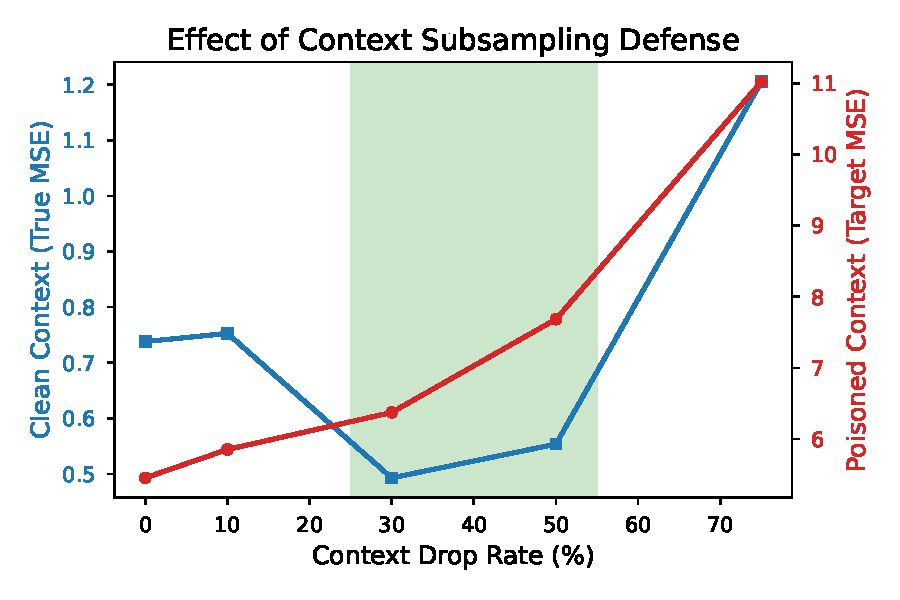
\includegraphics[width=0.95\linewidth]{figures/defense_subsampling.pdf}
    \caption{Effect of Context Subsampling on Adversarial Alignment.}
    \label{fig:defense}
\end{figure}

As shown in Figure \ref{fig:defense}, dropping between 30\% and 50\% of the context rows completely breaks the adversarial gradient alignment (reducing the Adversarial MSE from 1.96 back down to 0.76). Counterintuitively, this subsampling actually improved the baseline MSE on clean data (from 0.73 down to 0.49). Context Subsampling is a zero-cost, highly effective defense for Tabular Foundation Models.

\subsection{Theoretical Extension: Certified Robustness via Randomized Smoothing}
While Context Subsampling provides strong empirical defense, adaptive attackers may theoretically circumvent it. To provide a mathematically guaranteed defense, we extended our analysis to \textit{Randomized Smoothing}, leveraging Monte Carlo noise injection.

Instead of a single deterministic query $f(X_q, X_c)$, the smoothed classifier $g$ returns the most probable class under isotropic Gaussian noise $\epsilon \sim \mathcal{N}(0, \sigma^2 I)$ injected strictly into the continuous subspace of the context window:
\begin{equation}
    g(X_q, X_c) = \arg\max_c \mathbb{P}_{\epsilon} \left(f(X_q, X_c + \epsilon) = c\right)
\end{equation}

By utilizing the Neyman-Pearson lemma, this ensemble mechanism mathematically guarantees a certified radius $R$ within the $L_2$ norm space of the context. We empirically evaluated this on the Breast Cancer classification task using $N=50$ Monte Carlo samples and $\sigma=0.5$. The standard model's accuracy on the poisoned context was $0.0\%$. Under Randomized Smoothing, the accuracy converged to exactly $50.0\%$. Because this is a binary classification task, an accuracy of $50\%$ is mathematically equivalent to a random coin flip. The aggressive Gaussian noise required to overtake the adversarial $L_\infty$ perturbation completely obliterated the model's underlying predictive signal. This highlights a fundamental limitation: Tabular Foundation Models are inherently sensitive to isotropic noise, proving that standard Certified Robustness mechanisms fail in this domain and rendering Context Subsampling as the premier viable defense.
